\documentclass{article}
\usepackage[utf8]{inputenc}
\usepackage{graphicx}
\usepackage{float}
\usepackage[font=footnotesize, labelsep=period]{caption}

\begin{document}

En la figura \ref{fig:convergencia_bo} se muestra la evolución del RMSE durante el proceso de optimización bayesiana.

\begin{figure}[H]
\centering
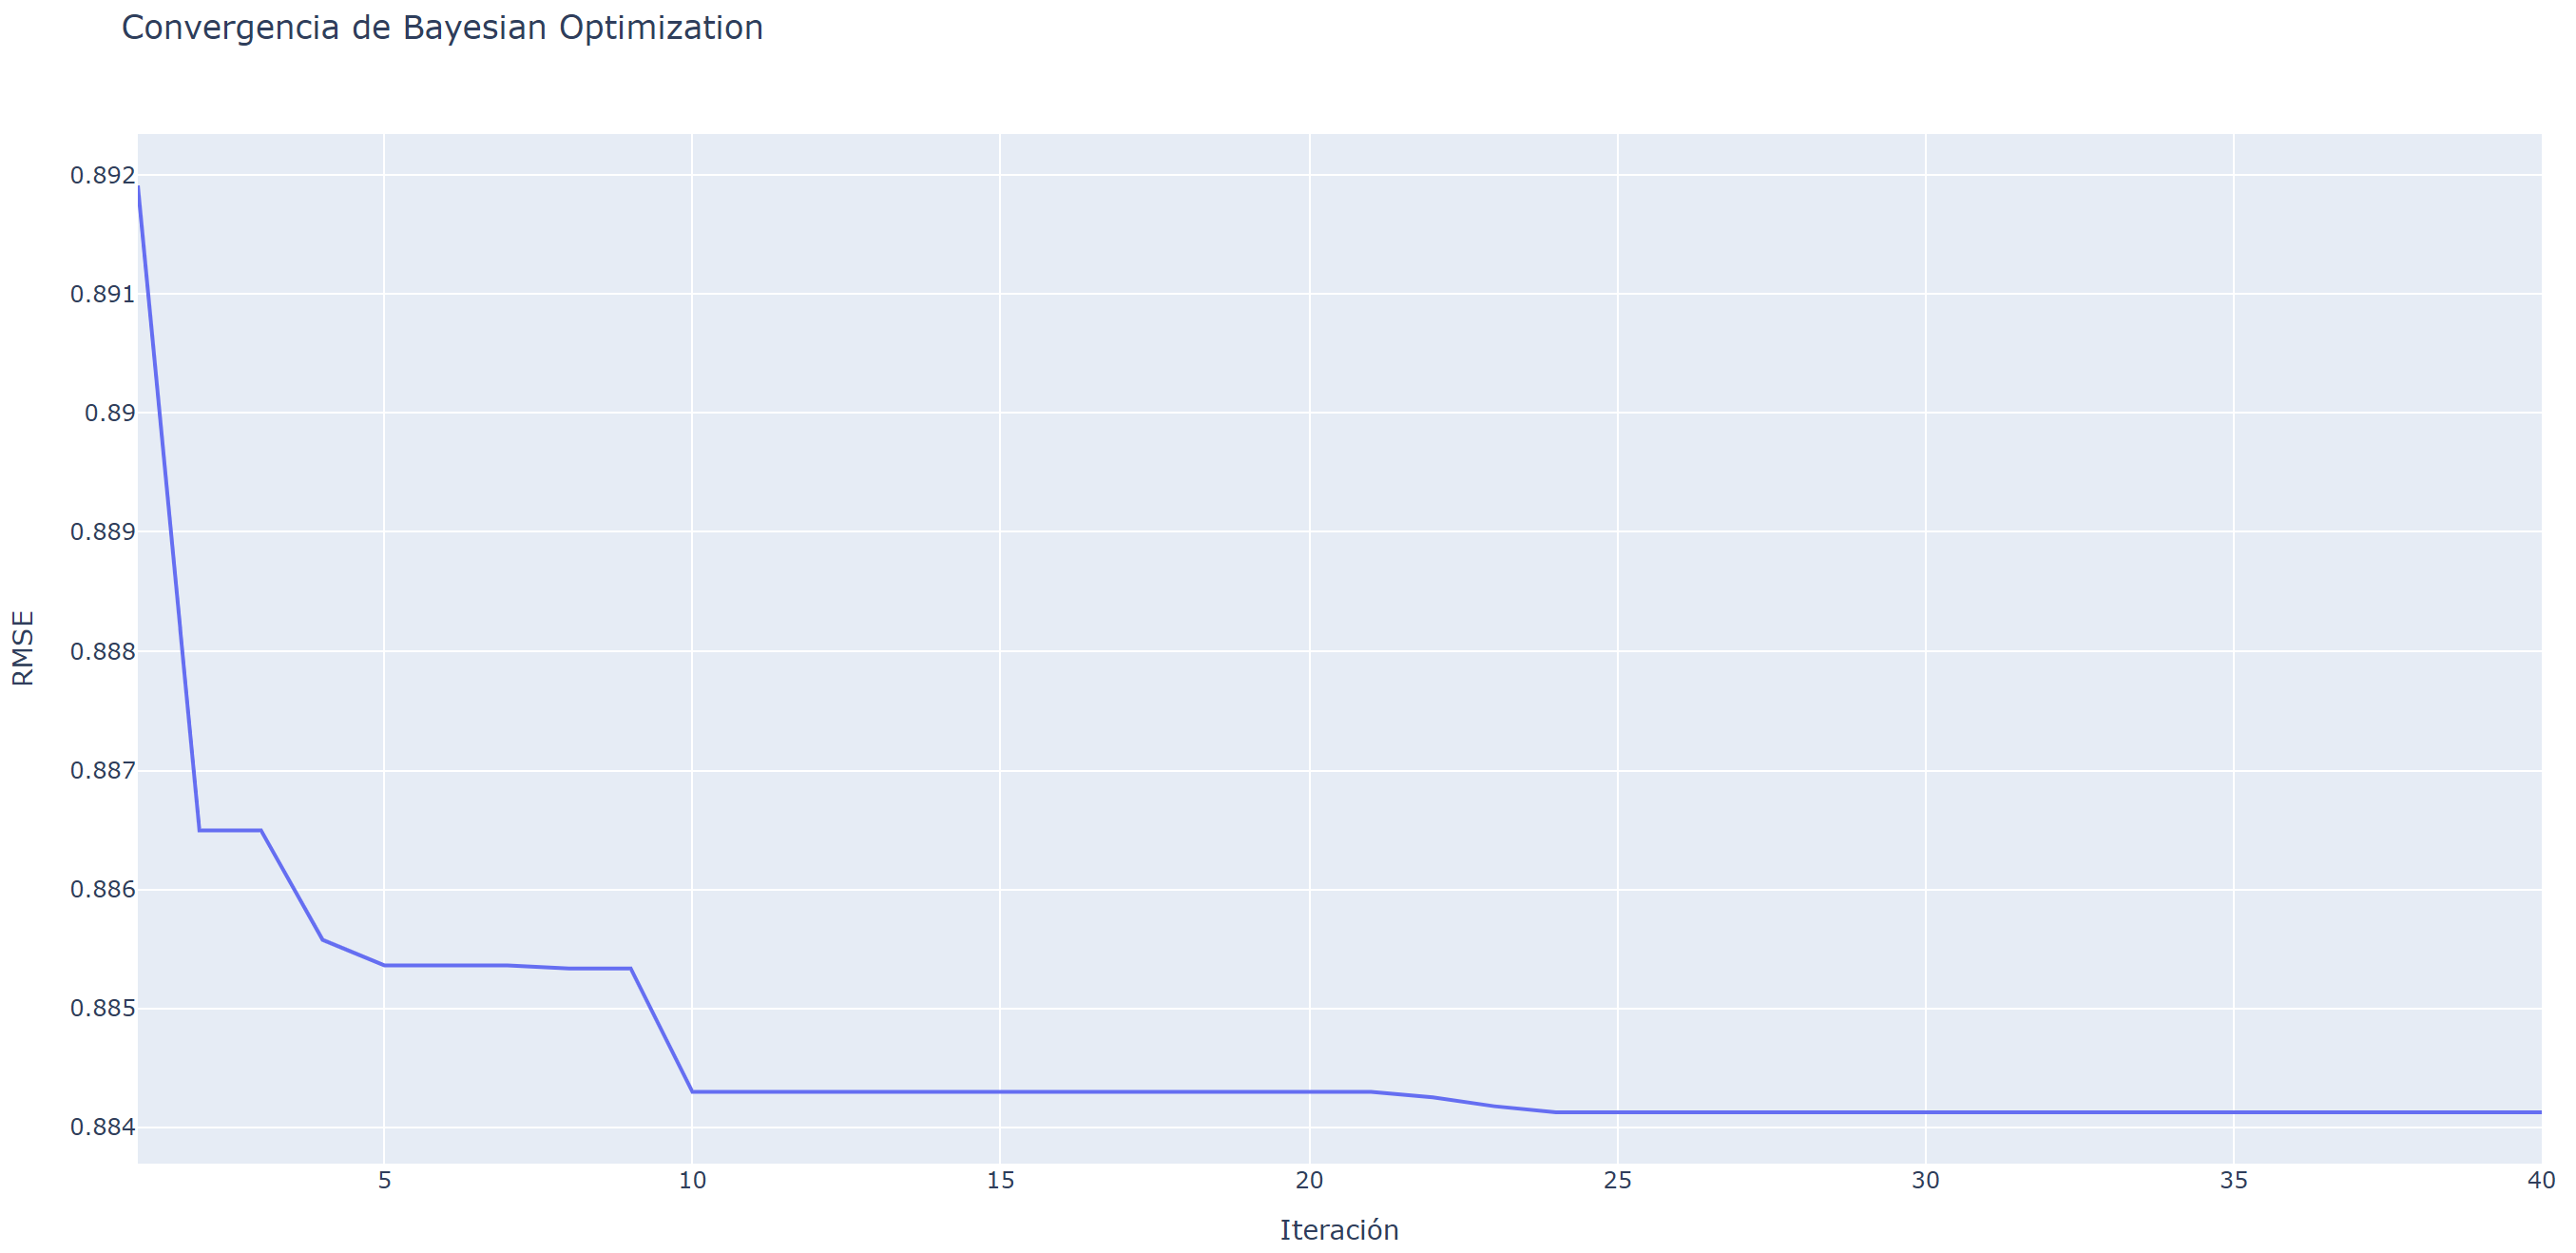
\includegraphics[width=0.47\textwidth]{fig_convergencia_bo.png}  % Cambia aquí la ruta si está en una subcarpeta
\caption{Convergencia de Bayesian Optimization}
\label{fig:convergencia_bo}
\end{figure}

\end{document}
